
% This LaTeX was auto-generated from an M-file by MATLAB.
% To make changes, update the M-file and republish this document.

\documentclass{article}
\usepackage{graphicx}
\usepackage{color}

\sloppy
\definecolor{lightgray}{gray}{0.5}
\setlength{\parindent}{0pt}

\begin{document}

    
    
\subsection*{Contents}

\begin{itemize}
\setlength{\itemsep}{-1ex}
   \item Set-up and motor variables
   \item Moments of Intertia and Damping due to load (average of all parts)
   \item Mathematical modeling of motor transfer function
\end{itemize}
\begin{verbatim}
%Control needs analysis of 12V Pittman 8224 motor with G35A wide-faced gear box
\end{verbatim}


\subsection*{Set-up and motor variables}

\begin{verbatim}
clc
clear all
Ke = 0.01;%[V/rad/s]
Kt = Ke;%Due to SI units
Km = Kt;%Therefore we have only one constant, a motor constant Km
Bm = 1.34e-6;% Viscous damping factor,[Nm*s/rad]
Jm = 1.62e-6;%Inertia of rotor, [kg*m^2]
La = 0.58e-3;%Armature Inductance, [H]
Ra = 1.17;%Armature Resistance, [Ohm]
n = 60.5;% Ratio of G35A gear box => wm/wl
Eff = 0.66;% Efficeincy of gear-box, losses due to gear box gear friction
neff = n*Eff;%Effective gear ratio of gear-box due to friction losses
Inl = 0.37;%No load current draw[A]
Tloss = Inl*Kt;% Torque loss due to the motor shaft [Nm]
\end{verbatim}


\subsection*{Moments of Intertia and Damping due to load (average of all parts)}

\begin{verbatim}
J_load = 0.0059;%[kg*m^2]
B_load = 0.0166;%[N*m*s/rad]
\end{verbatim}


\subsection*{Mathematical modeling of motor transfer function}

\begin{par}
Load is reffered to motor via effective gear ratio Model obtained from \begin{verbatim}Journey from Robot to Digital Human\end{verbatim}, pg. 298 By: Edward Y.L. Gu, Springer, 2013
\end{par} \vspace{1em}
\begin{verbatim}
Jeff = Jm + (J_load/(neff)^2);%Effective inertia experienced by motor
Beff = Bm + (B_load/(neff)^2);%Effective damping experienced by motor
num = [(-La*Tloss) (Ra+Km)];
den = [(Jeff*La) ((Jeff*Ra) + (Beff*La) - (Km*Tloss)) ((Beff*Ra) + (Km^2) - (Ra*Tloss*Km))];
Sys = tf(num, den)%System TF
% Transfer function:
%   -2.146e-006 s + 1.18
% ------------------------------------------
% 3.086e-009 s^2 - 3.077e-005 s + 7.046e-005
w_n = sqrt(((Beff*Ra) + (Km^2) - (Ra*Km*Tloss))/(Jeff*La))
% resonant frequnecy
% w_n =
%
%   151.1057
z = (0.5*((Jeff*Ra)+ (Beff*La) - (Km*Tloss))/sqrt(((Beff*Ra)+(Km^2)-(Ra*Km*Tloss))/(Jeff*La)))
%damping factor
% z =
%
%  -1.0181e-007

%Graph of system step response
figure(1);
step(Sys)
\end{verbatim}

        \color{lightgray} \begin{verbatim} 
Transfer function:
           -2.146e-006 s + 1.18
------------------------------------------
3.086e-009 s^2 - 3.077e-005 s + 7.046e-005
 

w_n =

  151.1057


z =

 -1.0181e-007

\end{verbatim} \color{black}
    
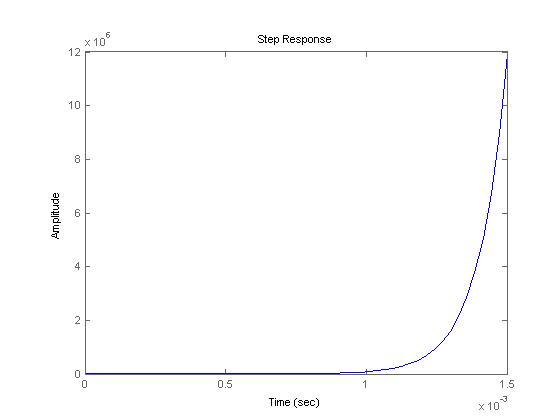
\includegraphics [width=4in]{PaulsMotorModeling_01.eps}



\end{document}
    
